\chapter{Implementation}
The virtual globe rendering system was implemented as a separate module, programmed in C++ for OpenSpace, which, if desired, can be opted out in CMake. The implementation defines a namespace with all the necessary data structures, classes and functionality specifically related to globe rendering.

The base of the globe renderer uses a modified version of Cozzi and Rings Chunked LOD algorithm. The globe is tessellated as an ellipsoid with a geometrical grid using geodetic map projection.

\begin{figure}[htbp]
    \centering
    \begin{subfigure}[bt]{0.8\textwidth}
        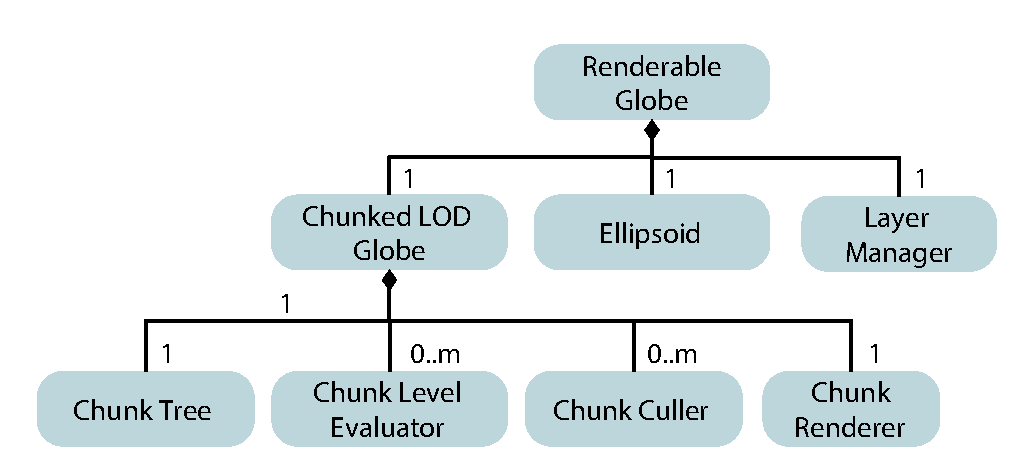
\includegraphics[width=\textwidth]{figures/implementation/renderable_globe.pdf}
    \end{subfigure}
    \caption{Overviewing class diagram of RenderableGlobe and its related classes.}
    \label{fig:renderableglobe}
\end{figure}

The full LOD rendering system required several components of different complexity to be implemented. These along with their puruposes are listed below.

\begin{enumerate}
	\item \textbf{Reference Ellipsoid}% - A small independent component for geometry calculations.
	\item \textbf{Chunked LOD}% - Hierarchically arranges Chunks in a quadtree where each Chunk represents a geographical region and can be rendered individually.
	\item \textbf{Reading and Tiling Image Data}% - A large component that takes care of concurrent texture fetching, georeferencing and tiling up textures to fit chunks. 
	\item \textbf{Providing Tiles}% - How to access different types of tiles.
	\item \textbf{Mapping Tiles onto Chunks}% - 
	\item \textbf{Managing Multiple Data Sources}% - Organizes different texture layers into categories and makes the texture data accessible for rendering. 
	\item \textbf{Chunk Rendering}% - 
\end{enumerate}



\section{Reference Ellipsoid}
The reference ellipsoid was implemented to handle all geographic related calculations.  These calculations include conversions between geodetic and cartesian coordinates and different kinds of projections onto the ellipsoid surface. These calculations are sped up by internal caching of a range of precalculated values. Cozzi and Ring provide a complete reference on the implementation \cite[p. 17]{cozzi11}.

The Ellipsoid uses several geographically related classes, which were used in multiple place within the implementation. These include:
\begin{enumerate}
	\item Angle - Handle angle related arithmetics, normalizations and abstract away unit (degrees and radians)
	\item Geodetic2 - Represents a 2D geodetic coordinate (latitude, longitude)
	\item Geodetic3 - Represents a 3D geodetic coordinate (latitude, longitude, altitude)
	\item GeodeticPatch - Represents a rectangular region in geodetic space
\end{enumerate}

\section{Chunked LOD}
The base of the chunked LOD algorithm revolves around the self updating chunk tree. The chunk tree is a data structure built up of chunk nodes which have the ability to split or merge dynamically. Besides storing four children chunk nodes, each chunk node stores a Chunk.

\subsection{Chunks}
As opposed to the definition of chunks in Theoretical Background, this implementation of chunks is very lightweight - it does not store any texture or triangle mesh data. Instead, it stores the information needed to query texture tiles from local in-memory caches. In the implementation suggested by Cozzi and Ring, terrain triangle meshes are stored in each chunk. In the case of this implementation however, all terrain is rendered using height mapped vertex grids. Thus there is no need for each chunk to store their own vertex arrays. Instead they can simply share one single instance of a vertex grid within a whole chunk tree. This of course also means that vertices need to be offset by height mapping on the GPU.

The most important part of the chunked LOD algorithm is the ability to dynamically select which chunks to split or merge. 

\subsection{Chunk Selection}
The chunk tree is automatically reshaped depending on the virtual camera. A Chunk node splits, merges or remain the same depending on the chunk's error metric for the current LOD. Three different approaches for calculating the error metric were implemented.

\subsubsection{By Distance}
By letting the error depend on the distance between the closest point on the chunk, an the camera $d$ as in Equation \ref{eq:loddistance}, the size of the chunks in screen space stays more or less constant.

\begin{equation}
	\label{eq:loddistance}
	e = l - log_2(\frac{s}{d})
\end{equation}
Where $e$ is the error, $l$ is the current level of the chunk, $s$ is a LOD scaling factor and $d$ is the distance between the closest point of the chunk and the camera. The closest point of the chunk can be either a corner or a point along one of the chunk edges. Using this distance as an error metric leads to bigger chunks farther from the camera where less detail is needed.


\subsubsection{By Projection Area}
Another error metric is the area that the chunk take up on the screen. The bigger the area, the higher the error. 

The error must not be dependent of the direction of the camera. This is because a chunk rendered on a multi screen display should not have different errors between two or more screens which might lead to different levels and tearing between screens. Therefore the chunk is projected on a unit sphere and not a view plane which would lead to view direction dependent desired levels.

\begin{figure}[htbp]
    \centering
    \begin{subfigure}[bt]{0.6\textwidth}
        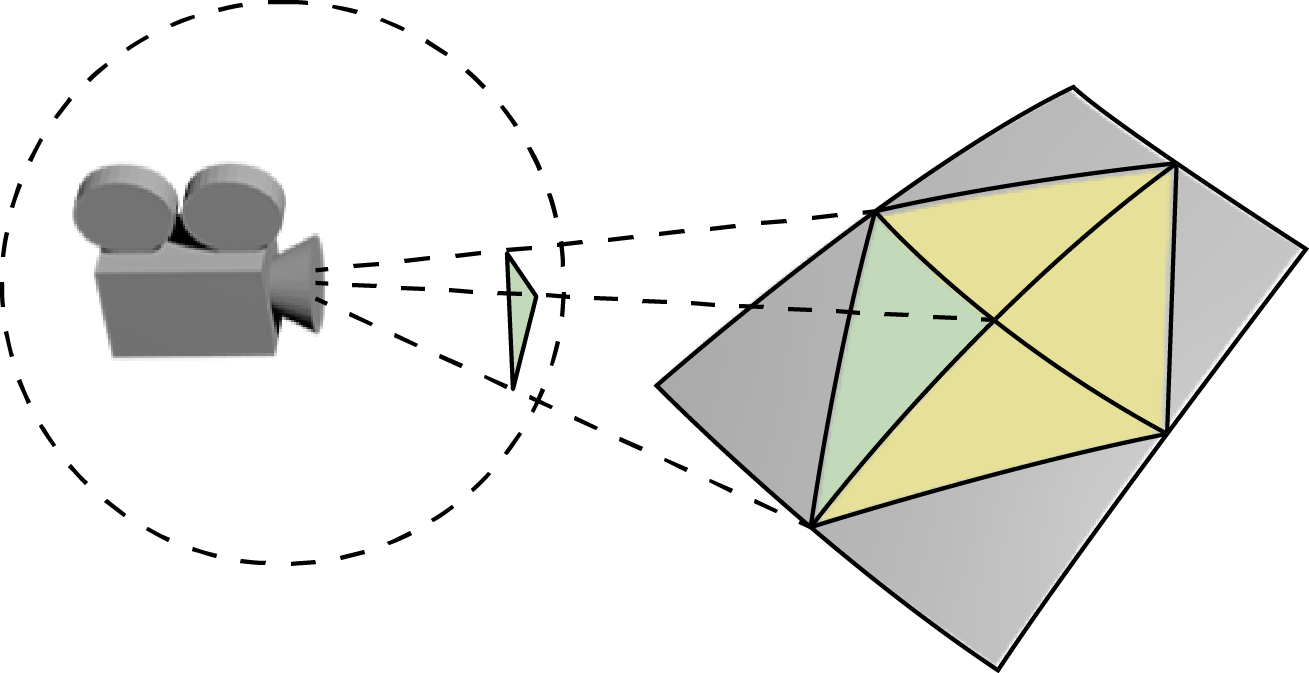
\includegraphics[width=\textwidth]{figures/implementation/chunklod/projectedarea.png}
    \end{subfigure}
    \caption{Chunk are projected onto a unit sphere}
    \label{fig:chunkprojarea}
\end{figure}

The projected area is a solid angle approximated by extracting three points on the chunk and projecting them on a unit sphere centered in the camera position. The three points define the closest of the four center triangles on the chunk, see Figure \ref{fig:chunkprojarea}. It is important that the triangle chosen for approximating the projected area can never have two vertices on the same upper or lower most edge. Such triangles (colored gray in Figure \ref{fig:chunkprojarea}) may have null areas at the poles, thus cannot be used to approxate the area of the full chunk.

The actual approximated solid angle is the projected triangle area multiplied by eight to accommodate a full chunk. This area is then subtracted by a constant value and scaled by a LOD scale factor to give similar LOD scaling as the distance dependent chunk selection.

\subsubsection{By Available Tile}
Splitting a chunk will not result in higher level of detail unless the corresponding higher level of detail tile data is also currently available for rendering. Therefore, the growth of the chunk tree can be limited by checking if there is any tile data there in the first place. This is useful in two scenarios:

\begin{enumerate}
\item Rendering of sparse map datasets which contain geographical regions where there are no data
\item Rendering of map datasets which are queried from remote servers - there will always be some delay where the queried map data is not yet available
\end{enumerate}

Being able to limit the chunk tree in these two scenarios, unnecessary chunk rendering calls can be avoided.

\subsection{Chunk Culling}
Given a chunk tree with chunks selected based on the camera position, each chunk can be tested using chunk cullers to determine if they are ``cullable'' and therefore can be set to invisible so that the chunk renderer will not bother in rendering them. The two implemented chunk cullers are the frustum culler and the horizon culler. They both rely on - and have access to - minimum and maximum values of the Chunk's height maps. 

\subsubsection{Frustum Culling}
The frustum culling is implemented by first calculating a convex bounding polyhedron for the chunk to be tested. The bounding volume is calculated on the fly and takes into account any enabled height maps used to displace the vertices, making sure it fully encapsulates the displaced chunk vertices. The polyhedron is built up of eight vertices which are transformed to normalized device coordinates (NDC). Once in NDC, an axis aligned bounding box (AABB) for the vertices is extracted. This AABB can then be tested against the screen bounds to determine if the chunk is outside the camera's field of view, and thus can be cullable. This is illustrated in Figure \ref{fig:frustumculling}.

\begin{figure}[htbp]
    \centering
    \begin{subfigure}[bt]{1.0\textwidth}
        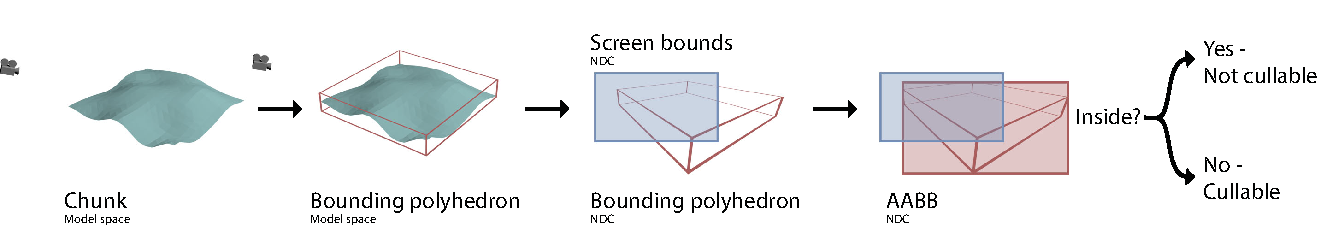
\includegraphics[width=\textwidth]{figures/implementation/chunklod/frustumculling.pdf}
    \end{subfigure}
    \caption{Frustum culling algorithm. The chunk cannot be culled.}
    \label{fig:frustumculling}
\end{figure}

\subsubsection{Horizon Culling}
Given an object in position $p$ with a bounding radius $r$, it can be determined if it is completely below the globe's horizon or not. The calculations are simplified by approximating the globe as a sphere using the minimum radius of its ellipsoid. Using the minimum radius and not a bigger number ensures that false occluding (chunks marked as invisible actually being visible) is not possible \cite[p. 393]{cozzi11}. The minimum allowed distance $l$ to the object can be calculated as the distance to the horizon $l_h$ added to the minimum allowed distance to the object from the horizon $l_m$. See equation horizon and figure horizon.

\begin{figure}[htbp]
    \centering
    \begin{subfigure}[bt]{0.25\textwidth}
        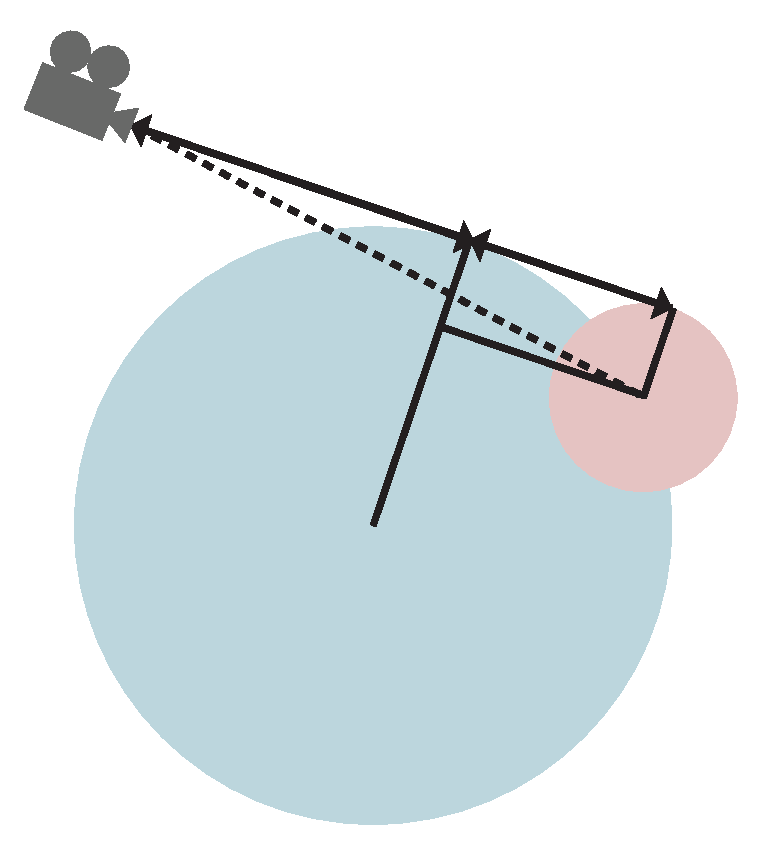
\includegraphics[width=\textwidth]{figures/implementation/chunklod/horizonculling.pdf}
    \end{subfigure}
    \caption{The horizon culling algorithm}
    \label{fig:horizonculling}
\end{figure}

When culling chunks, the closest position on the chunk is used as the position $p$ and the bounding height value as $r$.

\section{Reading and Tiling Image Data}
Fetching the right texture prepare it for rendering onto chunks is a fairly complicated process. Before digging into the details of this process, there are three concepts that need to be established, as they will be referenced to throughout the description of the texture pipeline. Those are:

\begin{enumerate}
	\item TileIndex - A tuple of three integers $(level, x, y)$ indexing a specific chunk region on the globe.
	\item RawTile - A texture carved out fit the geographical region of a specific chunk, along with some meta data. Each RawTile is associated with a TileIndex. 
	\item Tile - Just like RawTile, but the texture data is uploaded to the GPU and ready to use for rendering (unless it has a status not equal to ``OK''). As opposed to RawTiles, Tiles rely on a OpenGL context.	
\end{enumerate}

All Chunk height and texture data are represented using Tiles. Tiles are created on the client side (i.e. in OpenSpace) on the fly as they are needed. As the pixel data may need to be read from disk or even requested from remote servers, the whole tile preparation pipeline was implemented to be executed on separate threads in order to avoid blocking the rendering thread with image data reads. 

During the iterative process of developing the texture tile pipeline, three layers of abstraction were introduced in order to deal with the fairly high complexity. These are listed in Table \ref{table:tilepipeline}.

\begin{center}
  \begin{table}
  \caption[]{Abstraction layers used in the texture data pipeline}
    \label{table:tilepipeline}
  \begin{tabular}{| c | c | c | c |}
    \hline
      & \textbf{Component} 	& \textbf{Responsibility} & \textbf{Input --> Output} \\ \hline 
    1 & Async Tile Dataset 	& Async RawTile fetching  & TileIndex --> RawTile \\ \hline
    2 & Tile Dataset        & Tiling, georeferencing, preprocessing & TileIndex --> RawTile \\ \hline
    3 & GDAL         		& Image formats, I/O Operations & pixel region --> pixel data \\
    \hline
  \end{tabular}
  \end{table}
\end{center}

The subsequent sections of this chapter will cover each abstraction layer in more detail, starting from the bottom and going up the stack.


\subsection{GDAL}
Geospatial Data Abstraction Library (GDAL) is an open source library providing a uniform interface for reading, manipulating and writing geospatial data in the form of raster and vector data models \cite{gdal}. GDAL is used as an abstraction layer between all the map formats and the representation of Tile Datasets. It provides an interface allowing client code to specify pixel regions within a dataset to read from, independent of the underlying image format. Reading pixel data using the GDAL interface requires a set of parameters listed below and illustrated in Figure \ref{fig:gdalio}:

\begin{enumerate}
	\item A map overview to read pixel data from (if the dataset has overviews)
	\item A pixel region within that map overview to read pixels from
	\item The raster band(s) (e.g., color channels) to read
	\item A pointer to sufficient user allocated memory where GDAL can write the output of the read operation. 
	\item The pixel region to write the outputted pixel data. (The size of the pixel data to be written may differ from the pixel region to read from, in which case GDAL will resample and interpolate the pixel data automatically.)
	\item The layout (i.e., pixel spacing, raster band spacing and line spacing)
	\item The data type to retrieve the pixel data in
\end{enumerate}

\begin{figure}[htbp]
    \centering
    \begin{subfigure}[bt]{1.0\textwidth}
        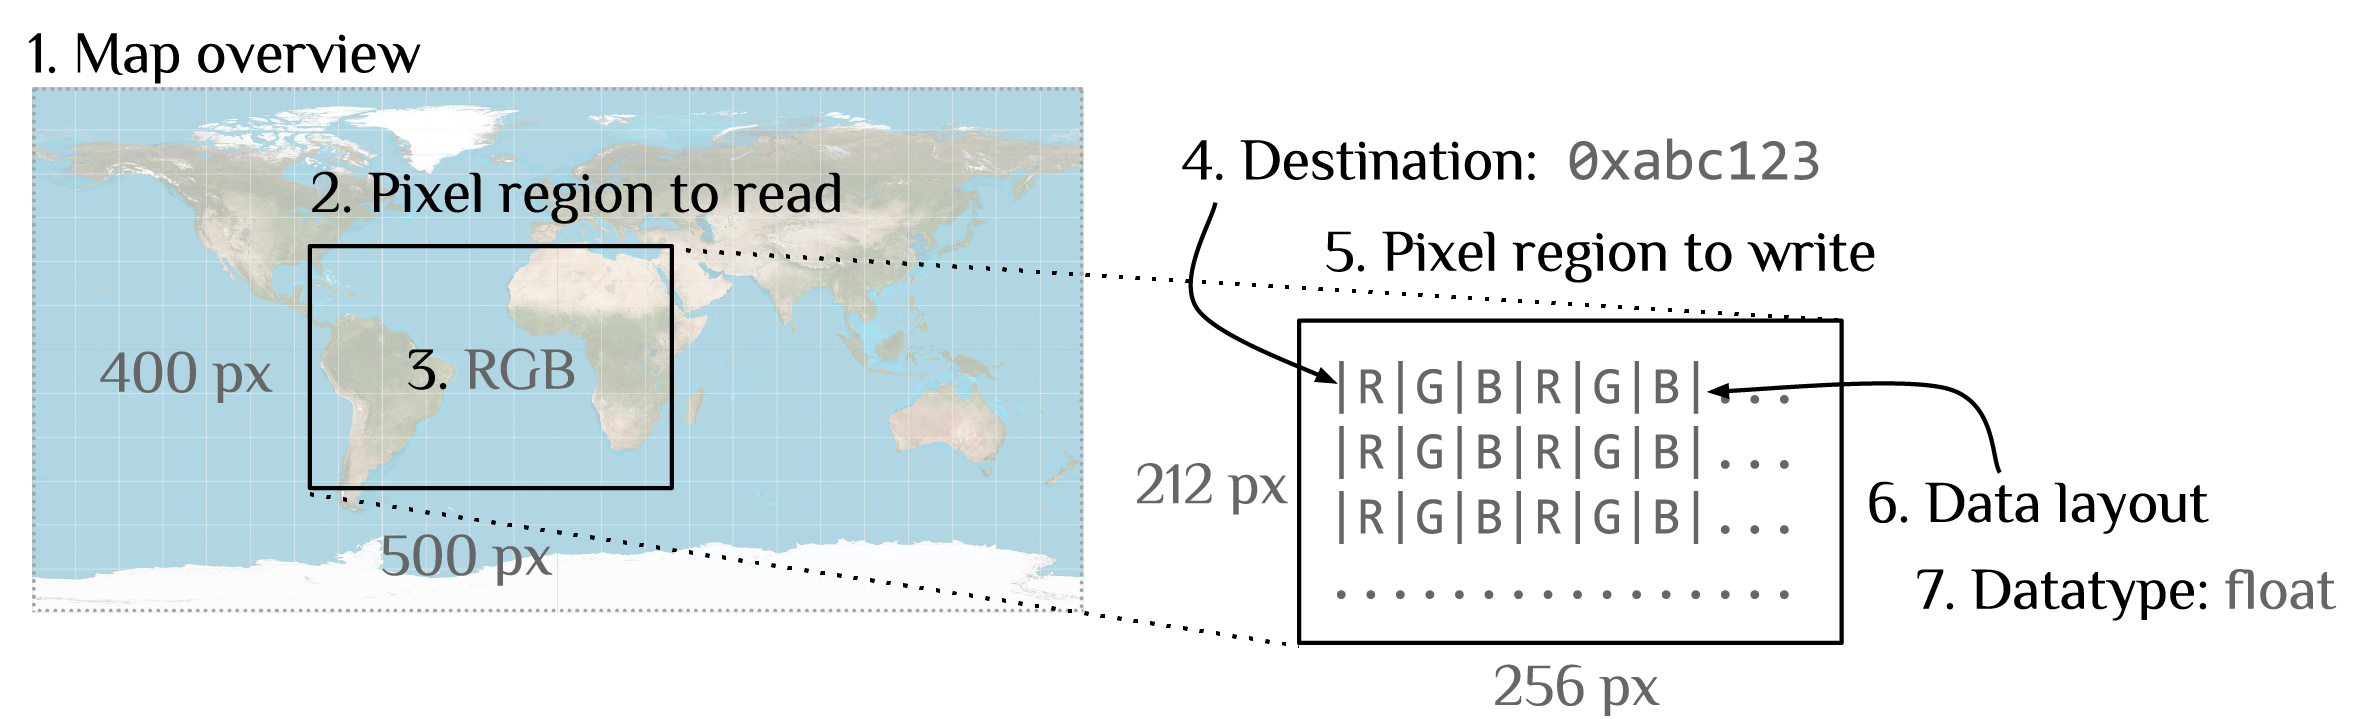
\includegraphics[width=\textwidth]{figures/implementation/pipeline/gdalio.png}
    \end{subfigure}
    \caption{The required GDAL raster IO parameters}
    \label{fig:gdalio}
\end{figure}

With the given input parameters shown in Figure \ref{fig:gdalio}, the resulting output would be the pixel data of the requested image region written with the pixel layout parameters to the provided memory block. The output is illustrated in Figure \ref{fig:gdalioresult}.

\begin{figure}[htbp]
    \centering
    \begin{subfigure}[bt]{0.5\textwidth}
        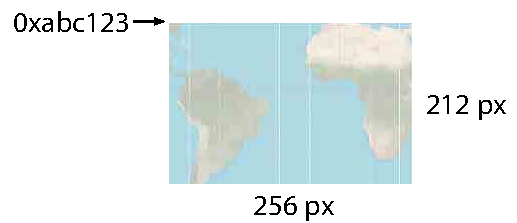
\includegraphics[width=\textwidth]{figures/implementation/pipeline/gdalioresult.pdf}
    \end{subfigure}
    \caption{Result of GDAL raster IO}
    \label{fig:gdalioresult}
\end{figure}

The using the RasterIO interface on an open GDAL dataset, the notion of image format is completely abstracted away. This is a great advantage which also allows GDAL to support sparse datasets. Appendix \textbf{majs} goes through a detailed example of how to use GDAL as an abstraction layer for sparse, non global, datasets such as local georeferenced image patches and use them in our globe browsing software.

GDAL also provides the coefficients of a geo-transform which defines the mapping from pixel coordinates to georeferenced coordinates.

\subsection{Tile Dataset}
Tile datasets carves out Raw tiles from GDAL datasets based on a Tile index. Along with the pixel data, the served Raw tiles also contain some metadata. The metadata includes an error code if something went wrong during the pixel reading process and some basic information about the read pixel data, such as minimum and maximum pixel values. Figure \ref{fig:tiledataset} illustrates how the process from Tile index to raw Tile is carried out. 

\begin{figure}[htbp]
    \centering
    \begin{subfigure}[bt]{0.8\textwidth}
        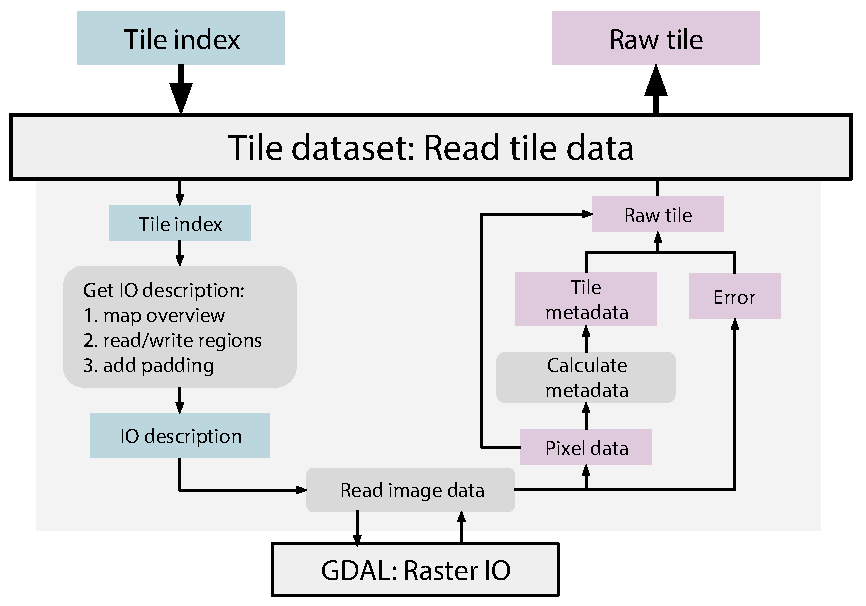
\includegraphics[width=\textwidth]{figures/implementation/pipeline/tiledataset.pdf}
    \end{subfigure}
    \caption{Tile datasets reads tiled pixel regions.}
    \label{fig:tiledataset}
\end{figure}

In Figure \ref{fig:tiledataset}, there are three gray subroutines; $Get IO description$, $Read image data$ and $Calculate metadata$. These subroutines are explained below.

\subsubsection{Get IO Description}
The IO Description contains all tile specific information needed to perform a map read request using GDAL. This includes the pixel region to read, and where to store the result, as described in the GDAL subsection above. The derivation of this information is summarized the follow steps, and illustrated in Figure \ref{fig:getiodescription}.

\begin{enumerate}
\item Calculate Geodetic patch from Tile index
\item Calculate Geodetic patch's pixel coordinates in map pixel space
\item Calculate a suitable map overview
\item Transform pixel region to map overview
\item Add padding to the down scaled pixel region
\item Finalize the gatherd to an IO description object.
\end{enumerate}

\begin{figure}[htbp]
    \centering
    \begin{subfigure}[bt]{0.9\textwidth}
        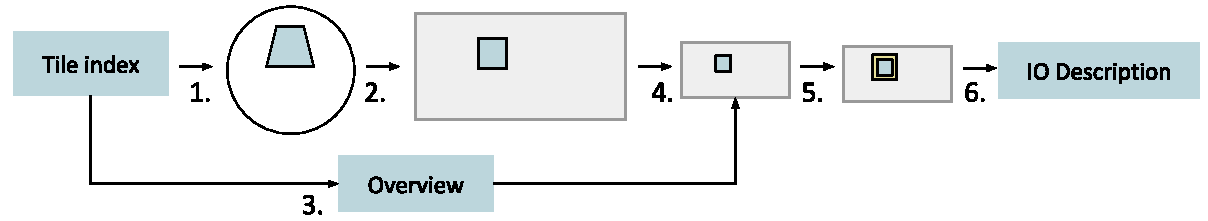
\includegraphics[width=\textwidth]{figures/implementation/pipeline/getiodescription.pdf}
    \end{subfigure}
    \caption{Overview of the calculation of an IO description}
    \label{fig:getiodescription}
\end{figure}

% @TODO
In the scheme in Figure IO Description, step one is done as described in theoretical background, eqation wat is defined under section hej. 
Calculating the corresponding GDAL overview is done according to

\begin{equation}
\label{eq:overview}
Overview(level) = N - level - 1 - log_2(size_{tile} / size_{map})
\end{equation}

Where $level$ is given by the provided Tile index, $N$ is the total number of overviews in the dataset, $size_{tile}$ is a configurable constant defining the preferred pixel size of a tile and $size_{map}$ is the size of the full map in pixels. The sizes can be either along the x or y axis, but does not matter when using square tiles and maps. In the implementation x is used.

Pixel coordinates can easily be transfomed across map levels:

\begin{equation}
\label{eq:overview}
P_{n} = P_{m} * 2^{m-n}
\end{equation}

Where $n$ is the destination map overview and $m$ is the source map overview. This is used for downscaling the pixel region in step 4, where $n$ is the calculated suitable overview and $m$ is zero (i.e. the full map). 

Padding is added to the pixel region in order to do correct interpolation of pixel values across different tiles later during rendering. However, this may cause the pixel region to extend outside the map region. Therefor the last finalize step also handles wrapping of the pixel regions before return the final IO description. The wrapping used is a CPU implementation of $GL\_REPEAT$.

\subsection{Tile Meta Data}
As mentioned, tile datasets can be configured to calculate some metadata on the fly based on the pixel data that has been read. This information cannot be requested directly from GDAL, so this had to be implemented by explicitly looping through all the pixel values an extra time client side. In this case, raw tiles will be served with some additional information. The metadata includes minimum and maximum pixel values within the pixel data and whether or not the pixeldata contains missing-data values. Having access to minimum and maximum values for height layer tiles is required for the culling to be performed correctly since the cullers rely on having bounding boxes for the chunks.

\subsection{Summary}
To summarize, the implementation of TileDataset allow reading pixeldata from a GDAL dataset corresponding to a specific TileIndex, along with some metadata unless opted out. The RawTiles that are served are padded for correct interpolation avoiding visible edges in the texture between tiles. RawTiles are not available for rendering since the data is not yet on the GPU.

\section{Async Tile Dataset}
Async tile datasets utilize a shared thread pool and own a tile dataset. It provides a concurrent job posting interface for concurrent reads within the tile dataset. It has two important methods: 1) enqueueTileReadJob and 2) getFinishedTileReadJobs. Reading raw tiles on separate threads ensures that the render thread will not be delayed by image data requests, see Figure \ref{fig:asynctiledataset}.

\begin{figure}[htbp]
    \centering
    \begin{subfigure}[bt]{0.7\textwidth}
        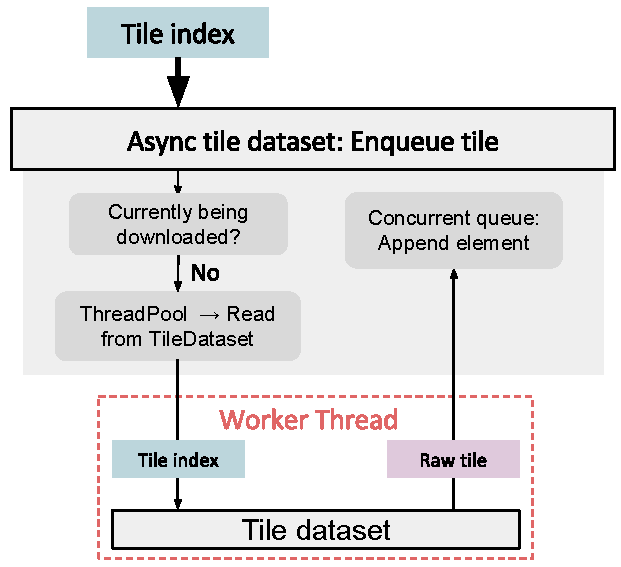
\includegraphics[width=\textwidth]{figures/implementation/pipeline/asynctiledataset.pdf}
    \end{subfigure}
    \caption{Asynchronious reading of Raw tiles.}
    \label{fig:asynctiledataset}
\end{figure}

\begin{figure}[htbp]
    \centering
    \begin{subfigure}[bt]{0.7\textwidth}
        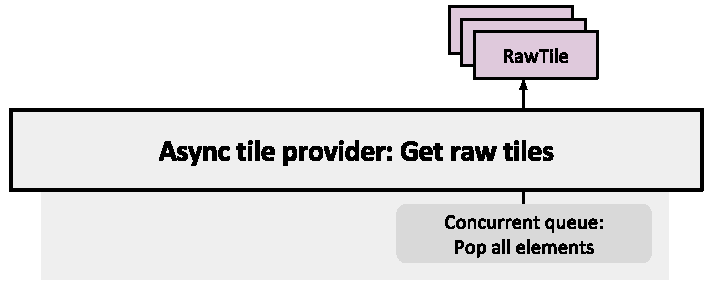
\includegraphics[width=\textwidth]{figures/implementation/pipeline/asynctiledataset2.pdf}
    \end{subfigure}
    \caption{Retrieving finished Raw tiles.}
    \label{fig:asynctiledataset2}
\end{figure}

The Async tile dataset internally keeps track of what tile indices it has enqueued and what tile index pixel regions are currently being read. If a pixel region for a specific Tile index already is currently being read, the request is simply ignored.

\begin{figure}[htb]
\centering
\caption{<Caption here>}
\end{figure}

\subsection{<Sub-section title>}

\section{<Section title>}

